\chapter{Thiết kế và hiện thực}
\label{chap:design_implementation}

Chương này trình bày kiến trúc hệ thống, quyết định thiết kế và chi tiết hiện thực của framework triển khai nhận dạng hoạt động trên thiết bị biên. Các thuật toán và cơ sở lý thuyết đã được trình bày trong Chương~\ref{chap:methodology}; chương này tập trung vào \textbf{kỹ thuật phần mềm}, \textbf{mô-đun hóa}, và \textbf{quy trình triển khai} của hệ thống thực tế. Framework được xây dựng dựa trên nguyên tắc tách biệt vai trò (separation of concerns): mỗi module chịu trách nhiệm một giai đoạn rõ ràng trong pipeline từ dữ liệu thô đến mã triển khai, đảm bảo tính mở rộng và khả năng bảo trì.

\section{Kiến trúc hệ thống}
\label{sec:system_architecture}

\subsection{Ngăn xếp công nghệ và môi trường phát triển}
\label{subsec:tech_stack}

Framework được triển khai dưới dạng ứng dụng web một trang (single-page web application) với các thành phần công nghệ sau:

\paragraph{Ngăn xếp phần mềm}
\begin{itemize}
    \item \textbf{Python 3.10}: ngôn ngữ lập trình chính, được chọn vì hệ sinh thái học máy phong phú và khả năng tích hợp nhanh giữa các thư viện khác nhau.
    \item \textbf{Dash 2.14}: framework giao diện web dựa trên Flask và Plotly. Dash cung cấp mô hình lập trình khai báo (declarative) với callback pattern, cho phép xây dựng giao diện tương tác phức tạp mà không cần JavaScript thủ công.
    \item \textbf{scikit-learn 1.3}: triển khai các thuật toán học máy truyền thống (Random Forest, SVM, MLP). Thư viện cung cấp API nhất quán và hiệu năng đã được tối ưu hóa.
    \item \textbf{PyTorch 2.x}: framework học sâu cho huấn luyện mô hình MLP và CNN. PyTorch được chọn vì API linh hoạt, hỗ trợ tốt cho tùy chỉnh kiến trúc, và khả năng xuất mô hình sang ONNX/TFLite.
    \item \textbf{NumPy/Pandas}: xử lý dữ liệu số học và cấu trúc dạng bảng. Pandas DataFrame cung cấp giao diện thuận tiện cho thao tác chuỗi thời gian và trích xuất đặc trưng.
    \item \textbf{Plotly}: thư viện trực quan hóa tương tác, hỗ trợ drag-and-drop selection và real-time updates trong giao diện Dash.
    \item \textbf{Jinja2}: template engine để sinh mã C/C++ và Arduino từ các mẫu tham số hóa, đảm bảo tính nhất quán cú pháp và dễ bảo trì.
\end{itemize}

\paragraph{Môi trường phát triển}
\begin{itemize}
    \item \textbf{Nền tảng phát triển}: Windows 11 workstation (Intel Core i7, 16GB RAM). Tuy nhiên, framework được thiết kế platform-agnostic và chạy được trên Linux/macOS mà không cần điều chỉnh.
    \item \textbf{Nền tảng chuẩn triển khai}: Seeed XIAO nRF52840 Sense (ARM Cortex-M4F @ 64MHz, 256KB RAM, 1MB Flash, LSM6DS3 IMU). Vi điều khiển này được chọn làm \textbf{nền tảng chuẩn đo benchmark} do: (1) tích hợp đầy đủ IMU 6-trục, (2) hiệu năng đại diện cho phân khúc MCU trung bình, (3) hỗ trợ Arduino và PlatformIO, và (4) giá thành thấp (\textasciitilde\$10 USD).
    \item \textbf{Công cụ biên dịch}: Arduino IDE 2.3 và PlatformIO cho biên dịch chéo (cross-compilation) sang ARM Cortex-M. Cả hai đều sử dụng GCC ARM Embedded Toolchain với flag tối ưu hóa \texttt{-O2} (cân bằng kích thước và tốc độ).
\end{itemize}

\subsection{Kiến trúc ứng dụng}
\label{subsec:app_architecture}

Framework áp dụng kiến trúc phân lớp rõ ràng với nguyên tắc \textit{separation of concerns}:

\paragraph{Cấu trúc thư mục}
\begin{verbatim}
app.py                  # Entry point, khởi tạo Dash app
├── layouts/            # UI components (Python code tạo Dash layout)
│   ├── data_upload.py
│   ├── preprocessing.py
│   ├── feature_engineering.py
│   ├── training.py
│   ├── code_generation.py
│   └── device_testing.py
├── callbacks/          # Business logic (xử lý sự kiện tương tác)
│   ├── *_callbacks.py  # Một file per tab, register_callbacks(app)
├── utils/              # Core algorithms (feature extraction, models)
│   ├── feature_extraction.py
│   ├── data_processing.py
│   ├── data_augmentation.py
│   └── edge_ml_model.py
├── deployment/         # Code generation subsystem
│   ├── code_generator_factory.py
│   ├── v2/             # Clean architecture với block pattern
│   │   ├── generator.py
│   │   ├── feature_block.py
│   │   ├── classifier_block.py
│   │   └── models/     # Model-specific blocks
│   └── converters/     # ONNX, TFLite converters
├── config/             # Configuration constants
└── persistent_data/    # Filesystem-based state
    ├── datasets/
    ├── windows/
    ├── training/
    ├── models/
    └── generated/
\end{verbatim}

\paragraph{Quy trình callback registration}
Dash sử dụng mô hình \textit{callback pattern} để đồng bộ giao diện và trạng thái. Mỗi module trong \texttt{callbacks/} định nghĩa một hàm \texttt{register\_callbacks(app)}, bên trong đó chứa tất cả decorator \texttt{@app.callback} liên quan đến tab tương ứng. Entry point \texttt{app.py} gọi tuần tự các hàm đăng ký này:

\begin{verbatim}
# app.py
from callbacks import (
    data_upload_callbacks,
    preprocessing_callbacks,
    feature_engineering_callbacks,
    # ...
)

data_upload_callbacks.register_callbacks(app)
preprocessing_callbacks.register_callbacks(app)
# ...
\end{verbatim}

Cách tổ chức này đảm bảo:
\begin{enumerate}
    \item \textbf{Tính module}: mỗi file callback độc lập, dễ bảo trì.
    \item \textbf{Tránh circular imports}: callbacks không import lẫn nhau, chỉ import từ \texttt{utils/} và \texttt{deployment/}.
    \item \textbf{Testability}: mỗi callback có thể kiểm thử riêng biệt bằng cách mock Dash context.
\end{enumerate}

\subsection{Quản lý trạng thái}
\label{subsec:state_management}

Framework sử dụng kết hợp hai cơ chế lưu trạng thái:

\paragraph{Hệ thống file (persistent\_data/)}
Dữ liệu trung gian giữa các giai đoạn được lưu dưới dạng file CSV, pickle (scikit-learn models) và joblib (model bundles):
\begin{itemize}
    \item \textbf{datasets/}: dữ liệu CSV gốc theo activity class.
    \item \textbf{windows/}: sliding windows đã sinh (pickle format).
    \item \textbf{training/}: feature matrices (CSV) và metrics.
    \item \textbf{models/}: model serialization (joblib) với dict keys chuẩn:
    \begin{itemize}
        \item \texttt{model}: trained model object (sklearn/PyTorch)
        \item \texttt{scaler}: StandardScaler fitted trên train set
        \item \texttt{label\_encoder}: mapping class names ↔ integers
        \item \texttt{feature\_names}: danh sách features theo thứ tự huấn luyện
        \item \texttt{model\_type}: string identifier (rf/svm/nn/cnn)
        \item \texttt{model\_params}: hyperparameters
        \item \texttt{performance\_metrics}: accuracy, F1, confusion matrix
    \end{itemize}
    \item \textbf{generated/}: mã nguồn triển khai theo cấu trúc \texttt{\{model\_type\}\_models/\{model\_name\}/}.
\end{itemize}

\paragraph{In-memory state (dcc.Store)}
Dash component \texttt{dcc.Store} lưu trạng thái session tạm thời (VD: metadata cột cảm biến, tần số lấy mẫu, danh sách segments đã chọn). State này được truyền giữa các callbacks trong cùng một session nhưng không persist sau khi reload trang.

\paragraph{Luồng dữ liệu}
Dữ liệu chảy qua pipeline như sau:
\begin{enumerate}
    \item \textbf{Tab 1 → Tab 2}: CSV files → \texttt{datasets/} → metadata in \texttt{dcc.Store}
    \item \textbf{Tab 2 → Tab 3}: Segments selection → sliding windows → \texttt{windows/\{dataset\_name\}.pkl}
    \item \textbf{Tab 3 → Tab 4}: Feature extraction → \texttt{training/\{dataset\_name\}\_train.csv}
    \item \textbf{Tab 4 → Tab 5}: Trained model → \texttt{models/\{model\_name\}.joblib}
    \item \textbf{Tab 5 → Tab 6}: Generated code → \texttt{generated/\{model\_type\}\_models/\{model\_name\}/}
\end{enumerate}

Thiết kế này cho phép người dùng quay lại bất kỳ bước nào để điều chỉnh mà không mất dữ liệu trung gian.

\section{Module quản lý dữ liệu}
\label{sec:data_management_module}

Module này (Tab 1 trong giao diện) chịu trách nhiệm tải dữ liệu cảm biến và kiểm tra trực quan chất lượng tín hiệu.

\subsection{Giao diện tải dữ liệu}
\label{subsec:data_upload_interface}

Người dùng tải lên nhiều file CSV, mỗi file chứa dữ liệu cho một activity class. Framework tự động phát hiện cấu trúc cột dựa trên quy ước đặt tên:
\begin{itemize}
    \item \textbf{Gia tốc kế}: \texttt{aX}, \texttt{aY}, \texttt{aZ} hoặc \texttt{AccX}, \texttt{AccY}, \texttt{AccZ}
    \item \textbf{Con quay hồi chuyển}: \texttt{gX}, \texttt{gY}, \texttt{gZ} hoặc \texttt{GyroX}, \texttt{GyroY}, \texttt{GyroZ}
    \item \textbf{Timestamp}: \texttt{time}, \texttt{timestamp}, \texttt{Time(s)} (optional, dùng để tính tần số lấy mẫu)
\end{itemize}

Thuật toán phát hiện cột:
\begin{verbatim}
def detect_sensor_columns(df):
    acc_patterns = ['aX', 'aY', 'aZ', 'AccX', 'AccY', 'AccZ', ...]
    gyro_patterns = ['gX', 'gY', 'gZ', 'GyroX', 'GyroY', 'GyroZ', ...]
    
    acc_cols = [c for c in df.columns if c in acc_patterns]
    gyro_cols = [c for c in df.columns if c in gyro_patterns]
    
    # Fallback: match columns chứa substring 'acc' hoặc 'gyro'
    if not acc_cols:
        acc_cols = [c for c in df.columns if 'acc' in c.lower()]
    # ...
    
    return acc_cols, gyro_cols
\end{verbatim}

\subsection{Trực quan hóa tín hiệu đồng bộ}
\label{subsec:signal_visualization}

Sau khi tải dữ liệu, framework hiển thị biểu đồ tín hiệu cho tất cả các trục cảm biến. Biểu đồ sử dụng Plotly \texttt{make\_subplots} với shared x-axis để đồng bộ zoom và pan giữa các trục:

\begin{verbatim}
fig = make_subplots(
    rows=6, cols=1, shared_xaxes=True,
    subplot_titles=['aX', 'aY', 'aZ', 'gX', 'gY', 'gZ']
)
for i, col in enumerate(sensor_columns):
    fig.add_trace(go.Scatter(y=df[col], mode='lines'), row=i+1, col=1)
\end{verbatim}

Hình~\ref{fig:ui_data_upload} minh họa giao diện này. Trực quan hóa này cho phép người dùng phát hiện các vấn đề chất lượng dữ liệu như:
\begin{itemize}
    \item \textbf{Nhiễu quá mức}: biên độ tín hiệu dao động lớn không đặc trưng cho hoạt động.
    \item \textbf{Outliers}: các spike đơn lẻ do lỗi cảm biến hoặc va chạm.
    \item \textbf{Saturation}: tín hiệu đạt giá trị max/min range của cảm biến (VD: $\pm 16g$).
    \item \textbf{Dữ liệu không đồng nhất}: tín hiệu chứa nhiều hoạt động khác nhau trong cùng một file.
\end{itemize}

\begin{figure}[H]
    \centering
    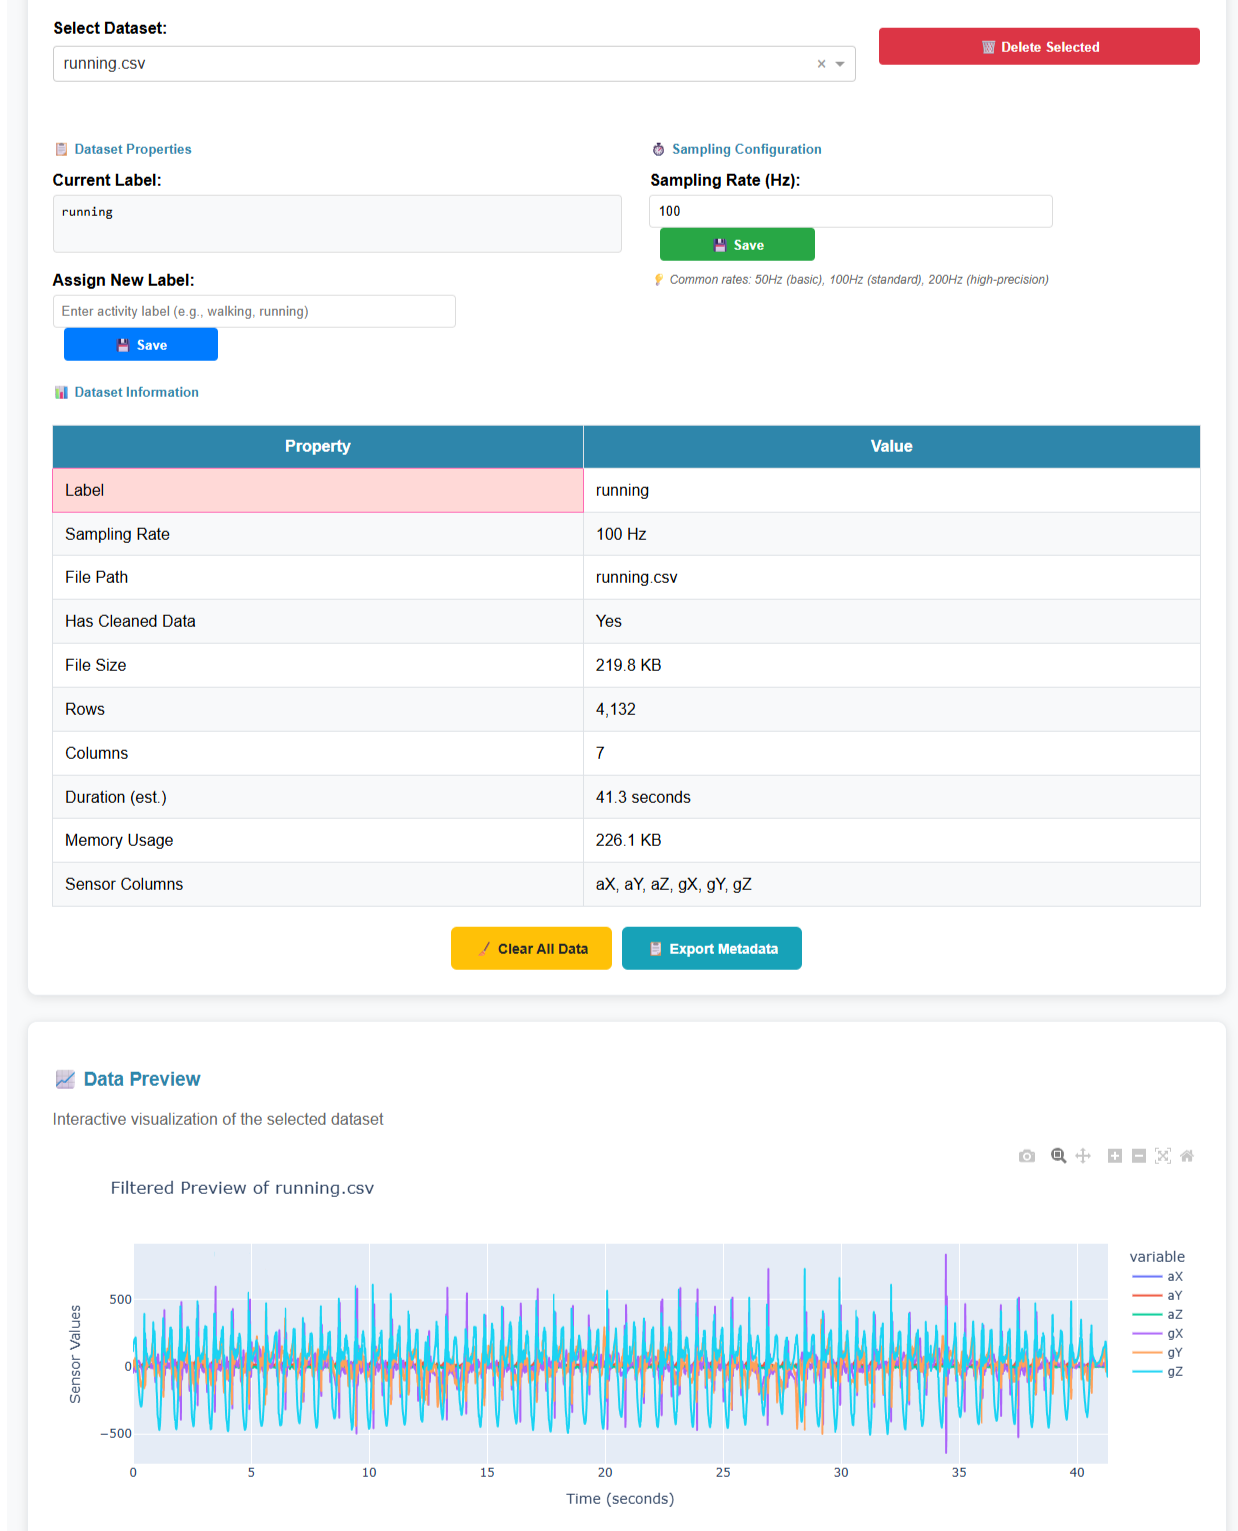
\includegraphics[width=0.95\textwidth]{figures/ui_data_upload.png}
    \caption{Giao diện tải lên và trực quan hóa dữ liệu cảm biến. Framework tự động phát hiện cấu trúc cột IMU và hiển thị biểu đồ tín hiệu đồng bộ trên tất cả các trục gia tốc kế và con quay hồi chuyển, cho phép kiểm tra trực quan chất lượng dữ liệu trước khi tiền xử lý.}
    \label{fig:ui_data_upload}
\end{figure}

\subsection{Phát hiện tần số lấy mẫu}
\label{subsec:sampling_rate_detection}

Framework tự động tính tần số lấy mẫu dựa trên cột timestamp:
\begin{verbatim}
if 'time' in df.columns or 'timestamp' in df.columns:
    time_col = 'time' if 'time' in df.columns else 'timestamp'
    time_diff = df[time_col].diff().dropna()
    sampling_rate = 1.0 / time_diff.mean()  # Hz
\end{verbatim}

Nếu không có cột timestamp, người dùng nhập tần số lấy mẫu thủ công. Tần số này được lưu trong metadata và nhúng vào mã triển khai dưới dạng hằng số \texttt{SAMPLE\_RATE\_HZ}.

\section{Module tiền xử lý tương tác}
\label{sec:preprocessing_module}

Module này (Tab 2) cung cấp giao diện kéo thả (drag-and-drop) để chọn các đoạn hoạt động đại diện trên biểu đồ tín hiệu, sau đó tự động sinh sliding windows từ các đoạn đã chọn.

\subsection{Giao diện lựa chọn đoạn tương tác}
\label{subsec:interactive_segment_selection}

Dash Plotly hỗ trợ \textit{editable shapes}: người dùng có thể vẽ hình chữ nhật (rectangle) trực tiếp trên biểu đồ để đánh dấu vùng quan tâm. Framework kích hoạt tính năng này qua thuộc tính \texttt{config.editable=True} và \texttt{newshape.drawdirection='horizontal'}.

Khi người dùng vẽ một rectangle, callback nhận được danh sách shapes:
\begin{verbatim}
@app.callback(
    Output('segment-store', 'data'),
    Input('signal-graph', 'relayoutData'),
    State('signal-graph', 'figure')
)
def update_segments(relayout_data, figure):
    if 'shapes' in relayout_data:
        shapes = relayout_data['shapes']
        segments = []
        for shape in shapes:
            x0 = int(shape['x0'])  # start sample index
            x1 = int(shape['x1'])  # end sample index
            segments.append({'start': x0, 'end': x1})
        return segments
\end{verbatim}

Framework kiểm tra các ràng buộc:
\begin{itemize}
    \item \textbf{Không chồng chéo}: các segment không được giao nhau.
    \item \textbf{Chiều dài tối thiểu}: mỗi segment phải có ít nhất \texttt{window\_size} mẫu để sinh được ít nhất 1 cửa sổ.
\end{itemize}

Hình~\ref{fig:ui_preprocessing} minh họa giao diện này.

\begin{figure}[H]
    \centering
    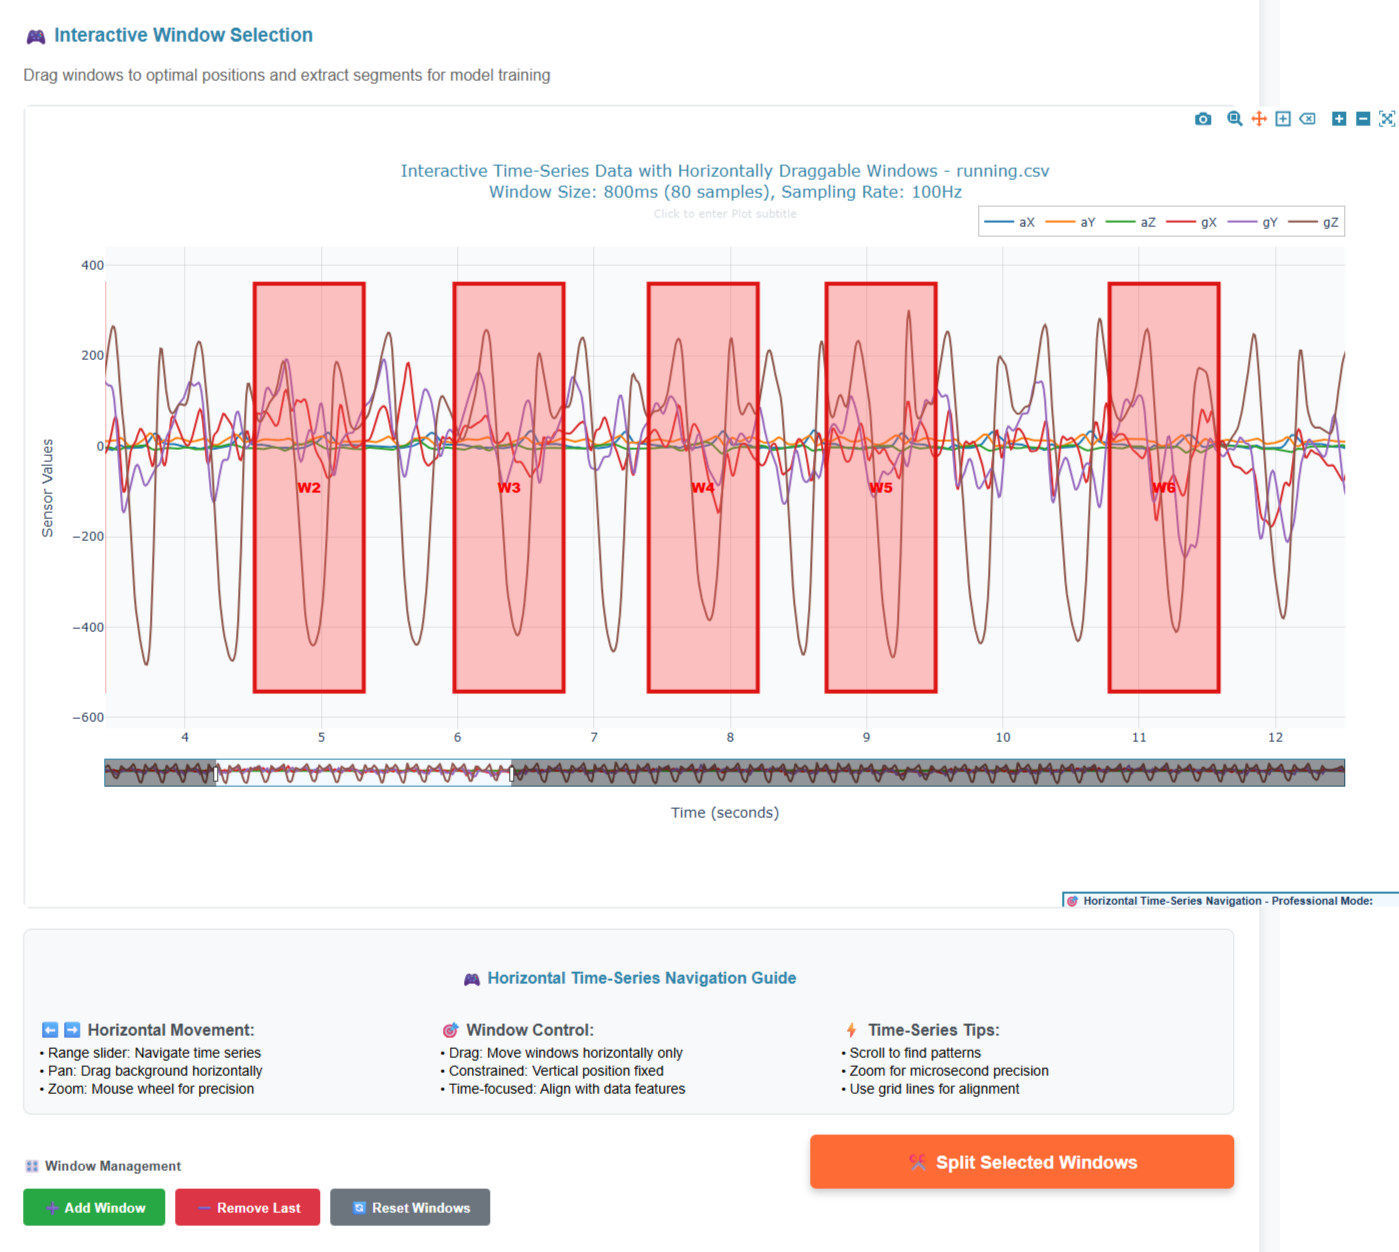
\includegraphics[width=0.95\textwidth]{figures/ui_preprocessing_draggable.png}
    \caption{Giao diện cửa sổ kéo thả tương tác. Người dùng kéo thả trực tiếp trên biểu đồ tín hiệu để xác định các đoạn hoạt động đại diện. Cửa sổ trượt tự động sinh các mẫu huấn luyện từ các đoạn đã chọn, kết hợp giữa kiểm soát thủ công và tự động hóa.}
    \label{fig:ui_preprocessing}
\end{figure}

\subsection{Sinh cửa sổ trượt}
\label{subsec:sliding_window_generation}

Từ mỗi segment, framework áp dụng sliding window với stride cố định:
\begin{verbatim}
def generate_windows(df, segments, window_size, stride):
    windows = []
    for seg in segments:
        start, end = seg['start'], seg['end']
        for i in range(start, end - window_size + 1, stride):
            window = df.iloc[i:i+window_size]
            windows.append(window)
    return windows
\end{verbatim}

Tham số mặc định:
\begin{itemize}
    \item \texttt{window\_size = 150} mẫu (1.5s ở 100Hz)
    \item \texttt{stride = 75} mẫu (50\% overlap)
\end{itemize}

Overlap 50\% được chọn để tăng số lượng mẫu huấn luyện đồng thời giữ sự đa dạng. Stride càng nhỏ (overlap càng lớn) càng tạo nhiều windows nhưng có nguy cơ overfitting do correlation giữa các windows liền kề.

\subsection{Trực quan hóa lọc tín hiệu}
\label{subsec:signal_filtering_viz}

Framework hỗ trợ ba phương pháp lọc tín hiệu (chi tiết thuật toán đã trình bày trong Chương~\ref{chap:methodology}):
\begin{enumerate}
    \item \textbf{Butterworth lowpass filter} (filtfilt for zero-phase)
    \item \textbf{Savitzky-Golay filter} (polynomial smoothing)
    \item \textbf{Kalman filter} (causal, exact training-deployment parity)
\end{enumerate}

Giao diện hiển thị overlay tín hiệu raw (màu xanh) và filtered (màu đỏ) để người dùng đánh giá hiệu quả lọc. Người dùng có thể điều chỉnh tham số (cutoff frequency, filter order, window length) và quan sát thay đổi real-time.

\section{Module trích xuất đặc trưng}
\label{sec:feature_engineering_module}

Module này (Tab 3) chịu trách nhiệm chuyển đổi cửa sổ tín hiệu thô sang feature vectors và chuẩn bị train/val/test splits.

\subsection{Chế độ trích xuất đặc trưng}
\label{subsec:feature_extraction_modes}

Framework hỗ trợ 6 chế độ feature extraction, mỗi chế độ tạo ra một tập đặc trưng khác nhau:

\begin{table}[H]
\centering
\caption{Các chế độ trích xuất đặc trưng và số lượng features}
\label{tab:feature_modes}
\begin{tabular}{@{}lll@{}}
\toprule
\textbf{Chế độ} & \textbf{Mô tả} & \textbf{Số features} \\ \midrule
\texttt{orientation\_invariant\_time\_only} & Magnitude stats (acc+gyro) + jerk & 33 \\
\texttt{orientation\_invariant} & Time + frequency domain magnitudes & 53 \\
\texttt{time\_domain} & Per-axis time stats + magnitudes & 90 \\
\texttt{all} & Time + frequency, per-axis + magnitudes & 156 \\
\texttt{frequency\_domain} & FFT, PSD, spectral features & 66 \\
\texttt{raw} & Cửa sổ tín hiệu raw (CNN input) & 6 channels \\ \bottomrule
\end{tabular}
\end{table}

\paragraph{Rationale cho orientation-invariant features}
Chế độ \texttt{orientation\_invariant} chỉ sử dụng các đặc trưng tính trên magnitude vectors ($\sqrt{x^2+y^2+z^2}$) thay vì per-axis features. Điều này đảm bảo mô hình không bị ảnh hưởng bởi định hướng lắp đặt cảm biến: đeo thiết bị ngang hoặc dọc, xoay 90° vẫn cho cùng một magnitude. Tuy nhiên, trade-off là mất thông tin về hướng chuyển động (VD: leo cầu thang khó phân biệt với xuống cầu thang chỉ dựa trên magnitude). Thực nghiệm cho thấy chế độ \texttt{time\_domain} (90 features) cân bằng tốt giữa độ chính xác và độ bền hướng.

\subsection{Tích hợp data augmentation}
\label{subsec:data_augmentation_integration}

Framework triển khai 5 phương pháp data augmentation cho dữ liệu IMU:

\begin{enumerate}
    \item \textbf{Jitter}: thêm Gaussian noise nhỏ vào tín hiệu ($\sigma = 0.05 \times \text{signal\_std}$).
    \item \textbf{Rotation}: xoay ngẫu nhiên hệ trục tọa độ 3D để mô phỏng thay đổi định hướng.
    \item \textbf{Scaling}: nhân tín hiệu với hệ số ngẫu nhiên (0.9--1.1) để mô phỏng biên độ chuyển động khác nhau.
    \item \textbf{Time warping}: kéo giãn hoặc nén trục thời gian (0.8--1.2$\times$) để mô phỏng tốc độ thực hiện hoạt động khác nhau.
    \item \textbf{Permutation}: hoán vị các sub-windows để phá vỡ sự phụ thuộc thứ tự thời gian (chỉ áp dụng cho hoạt động tuần hoàn như đi bộ).
\end{enumerate}

\paragraph{Class-aware augmentation}
Framework tự động phân loại hoạt động thành hai loại:
\begin{itemize}
    \item \textbf{Static/transition}: đứng yên, ngồi, nằm → KHÔNG áp dụng time warping và permutation (gây mất tính tự nhiên).
    \item \textbf{Dynamic/periodic}: đi bộ, chạy, leo cầu thang → áp dụng tất cả augmentation.
\end{itemize}

Phân loại dựa trên từ khóa trong tên activity:
\begin{verbatim}
STATIC_ACTIVITIES = ['still', 'stand', 'sit', 'lie', 'stationary']

def is_static_activity(activity_name):
    return any(keyword in activity_name.lower() 
               for keyword in STATIC_ACTIVITIES)
\end{verbatim}

Giao diện augmentation cho phép người dùng:
\begin{itemize}
    \item Kích hoạt/tắt từng phương pháp augmentation riêng biệt.
    \item Điều chỉnh augmentation factor (số lượng samples tăng thêm: 1$\times$, 2$\times$, 3$\times$).
    \item Xem phân phối class trước và sau augmentation để đảm bảo cân bằng.
\end{itemize}

Hình~\ref{fig:ui_feature_engineering} minh họa giao diện này.

\begin{figure}[H]
    \centering
    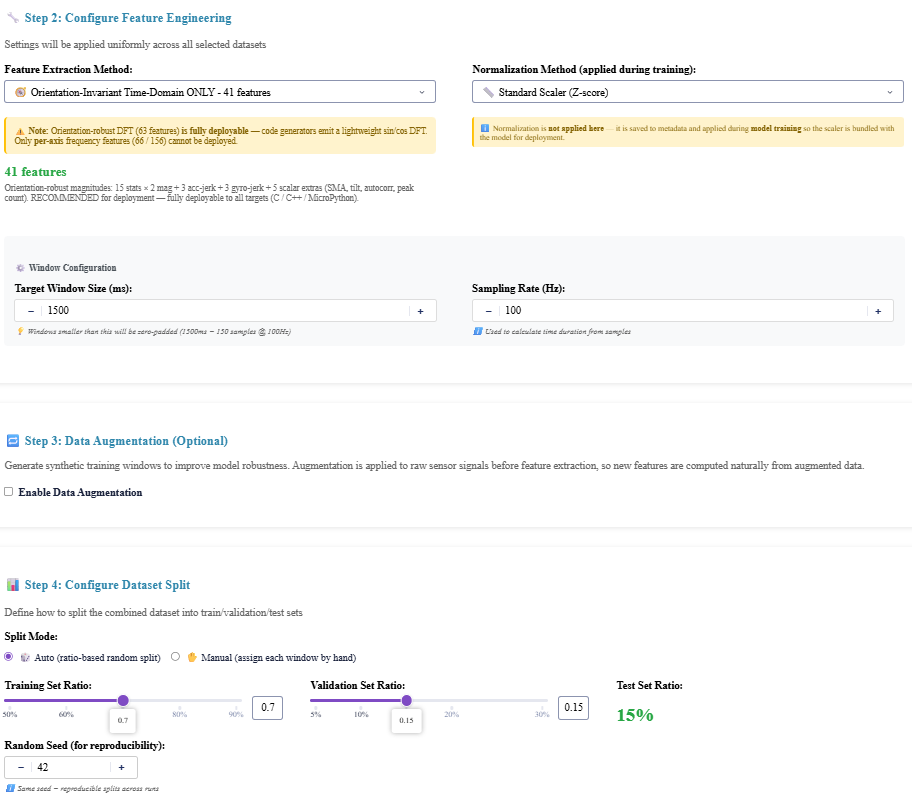
\includegraphics[width=0.95\textwidth]{figures/ui_feature_engineering.png}
    \caption{Giao diện trích xuất đặc trưng. Người dùng chọn loại đặc trưng (bất biến hướng, miền thời gian, miền tần số), cấu hình tăng cường dữ liệu nhận biết lớp, và phân chia dữ liệu huấn luyện/xác thực/kiểm tra với lấy mẫu phân tầng.}
    \label{fig:ui_feature_engineering}
\end{figure}

\subsection{Phân chia train/validation/test}
\label{subsec:train_val_test_split}

Framework sử dụng \texttt{sklearn.model\_selection.train\_test\_split} với stratified sampling để đảm bảo tỉ lệ class đồng đều giữa các tập:

\begin{verbatim}
# Split 1: train+val (80%) vs test (20%)
X_trainval, X_test, y_trainval, y_test = train_test_split(
    X, y, test_size=0.2, stratify=y, random_state=42
)

# Split 2: train (75% of trainval = 60% total) vs val (25% of trainval = 20% total)
X_train, X_val, y_train, y_val = train_test_split(
    X_trainval, y_trainval, test_size=0.25, stratify=y_trainval, random_state=42
)
\end{verbatim}

Kết quả cuối cùng: train 60\%, validation 20\%, test 20\%. Validation set được dùng cho hyperparameter tuning (GridSearchCV sử dụng cross-validation trên train+val), test set giữ nguyên không động đến cho đến khi đánh giá cuối cùng.

\section{Module huấn luyện mô hình}
\label{sec:training_module}

Module này (Tab 4) triển khai training pipeline với hyperparameter optimization và real-time monitoring.

\subsection{Lựa chọn thuật toán}
\label{subsec:algorithm_selection}

Framework hỗ trợ 6 thuật toán phân loại:

\begin{table}[H]
\centering
\caption{Thuật toán học máy được hỗ trợ}
\label{tab:algorithms}
\begin{tabular}{@{}llll@{}}
\toprule
\textbf{Thuật toán} & \textbf{Thư viện} & \textbf{Input} & \textbf{Triển khai} \\ \midrule
Random Forest & scikit-learn & Features & C++ native \\
SVM (RBF kernel) & scikit-learn & Features & C++ native \\
Neural Network (MLP) & scikit-learn & Features & C++ native \\
PyTorch MLP & PyTorch & Features & C++/TFLite \\
PyTorch 1D-CNN & PyTorch & Raw signals & C++/TFLite \\
PyTorch 2D-CNN & PyTorch & Raw signals (2D) & C++/TFLite \\ \bottomrule
\end{tabular}
\end{table}

\paragraph{Kiến trúc PyTorch models}
\begin{itemize}
    \item \textbf{PyTorch MLP}: 2 hidden layers với ReLU activation. Kích thước layer điều chỉnh theo số features: \texttt{[n\_features → 128 → 64 → n\_classes]}.
    \item \textbf{PyTorch 1D-CNN}: convolutional layers trên time dimension, kernel size = 5, 2 conv layers + pooling + fully connected. Input shape: \texttt{[batch, 6 channels, 150 timesteps]}.
    \item \textbf{PyTorch 2D-CNN (HARCNN2D)}: sử dụng Conv2D với kernel \texttt{3×n\_channels} để học correlation giữa các sensor axes. Input shape: \texttt{[batch, 1, 150 timesteps, 6 channels]} (reshape từ 1D signal).
\end{itemize}

Kiến trúc 2D-CNN đặc biệt hữu ích khi cần học mối quan hệ không tuyến tính giữa các trục cảm biến (VD: correlation giữa aX và gY trong động tác xoay).

\subsection{Tối ưu hóa siêu tham số}
\label{subsec:hyperparameter_optimization}

Framework tích hợp \texttt{GridSearchCV} từ scikit-learn với param grid mặc định cho từng thuật toán:

\paragraph{Random Forest}
\begin{verbatim}
param_grid = {
    'n_estimators': [50, 100, 200],
    'max_depth': [10, 20, None],
    'min_samples_split': [2, 5, 10]
}
\end{verbatim}

\paragraph{SVM}
\begin{verbatim}
param_grid = {
    'C': [0.1, 1.0, 10.0],
    'gamma': ['scale', 'auto', 0.01, 0.1]
}
\end{verbatim}

\paragraph{Neural Network}
\begin{verbatim}
param_grid = {
    'hidden_layer_sizes': [(100,), (128, 64), (256, 128)],
    'alpha': [0.0001, 0.001, 0.01],  # L2 regularization
    'learning_rate_init': [0.001, 0.01]
}
\end{verbatim}

GridSearchCV sử dụng 5-fold cross-validation trên train+validation set, chọn tổ hợp params có accuracy cao nhất, sau đó retrain trên toàn bộ train+val với params tối ưu.

\subsection{Theo dõi tiến trình real-time}
\label{subsec:realtime_monitoring}

Callback training sử dụng \texttt{dcc.Interval} component để cập nhật UI mỗi 2 giây trong quá trình huấn luyện. Thông tin hiển thị:
\begin{itemize}
    \item \textbf{Training progress}: phần trăm hoàn thành, thời gian đã trôi qua.
    \item \textbf{Current hyperparameters}: params đang thử nghiệm.
    \item \textbf{Best score so far}: accuracy cao nhất trong các trials đã hoàn thành.
    \item \textbf{Confusion matrix}: ma trận nhầm lẫn trên validation set, cập nhật sau mỗi trial.
\end{itemize}

Hình~\ref{fig:ui_training} minh họa giao diện này.

\begin{figure}[H]
    \centering
    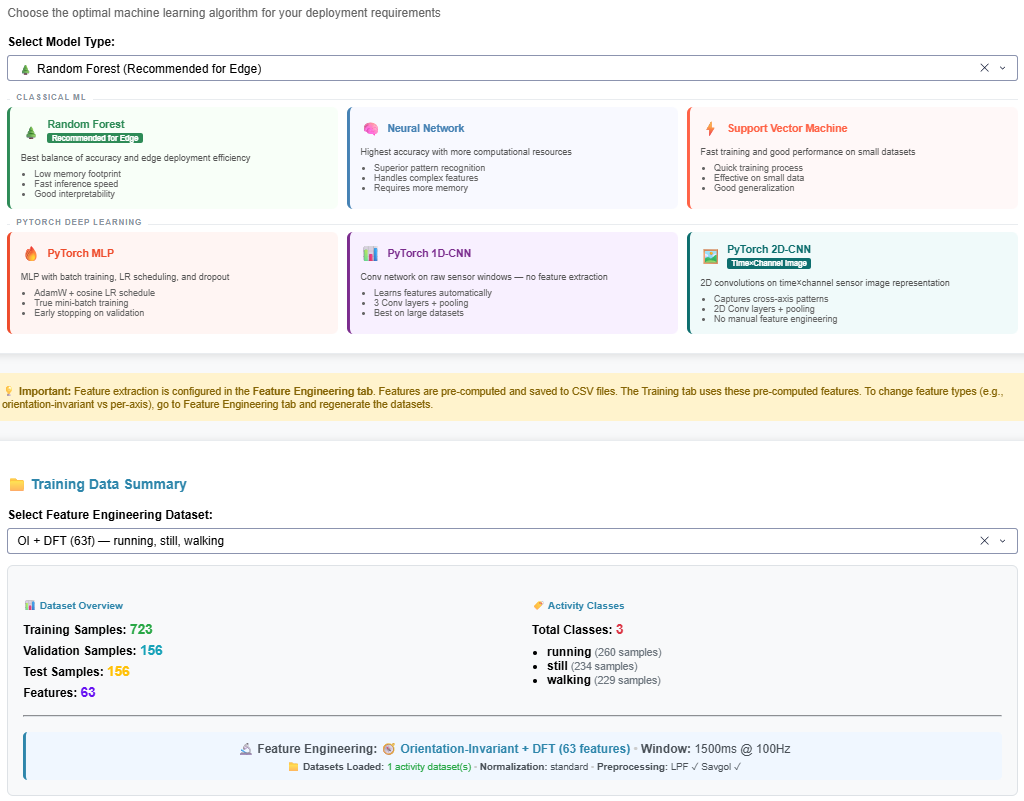
\includegraphics[width=0.95\textwidth]{figures/ui_training_config.png}
    \caption{Giao diện cấu hình huấn luyện mô hình. Người dùng chọn thuật toán, cấu hình tối ưu hóa siêu tham số với GridSearchCV, chiến lược cân bằng lớp, và theo dõi tiến trình huấn luyện thời gian thực.}
    \label{fig:ui_training}
\end{figure}

\subsection{Serialization mô hình}
\label{subsec:model_serialization}

Sau khi huấn luyện hoàn tất, framework serialize toàn bộ pipeline artifacts vào một file \texttt{.joblib}:

\begin{verbatim}
model_bundle = {
    'model': trained_model,  # sklearn/PyTorch model object
    'scaler': fitted_scaler,  # StandardScaler
    'label_encoder': le,  # class name ↔ integer mapping
    'feature_names': feature_columns,  # preserve order
    'model_type': 'random_forest',  # identifier
    'model_params': best_params,  # hyperparams
    'performance_metrics': {
        'accuracy': test_accuracy,
        'f1_score': f1_weighted,
        'confusion_matrix': cm,
        'classification_report': report_dict
    }
}

joblib.dump(model_bundle, f'models/{model_name}.joblib')
\end{verbatim}

Dict keys này là \textbf{chuẩn nội bộ} của framework. Module code generation dựa vào cấu trúc này để trích xuất parameters (VD: RF tree structures, NN weights) và sinh mã triển khai.

\section{Module tạo mã triển khai}
\label{sec:code_generation_module}

Module này (Tab 5) chịu trách nhiệm chuyển đổi trained model thành mã nguồn embedded C/C++ hoặc các định dạng khác (MicroPython, TFLite). Đây là thành phần phức tạp nhất của framework, vì phải đảm bảo \textbf{training-deployment parity}: mã được sinh ra phải tính toán đúng y hệt như Python pipeline.

\subsection{Kiến trúc Code Generator: Factory Pattern}
\label{subsec:code_generator_factory}

Framework sử dụng \textit{Factory Pattern} để định tuyến từ \texttt{(model\_type, target\_platform, deployment\_backend)} sang class generator phù hợp:

\begin{verbatim}
class CodeGeneratorFactory:
    @staticmethod
    def create_generator(model_data, platform, backend='direct'):
        model_type = model_data['model_type']
        
        if backend == 'tflite_micro':
            return TFLiteCodeGenerator(model_data, platform)
        
        if model_type == 'random_forest':
            return RandomForestCodeGenerator(model_data, platform)
        elif model_type in ['neural_network', 'pytorch_mlp']:
            return NeuralNetworkCodeGenerator(model_data, platform)
        elif model_type in ['pytorch_cnn', 'pytorch_cnn2d']:
            return CNNCodeGenerator(model_data, platform)
        elif model_type == 'svm':
            return SVMCodeGenerator(model_data, platform)
        # ...
\end{verbatim}

\subsection{Hệ thống phân cấp Generator}
\label{subsec:generator_hierarchy}

Framework áp dụng kiến trúc clean architecture với \textbf{block pattern}:

\paragraph{Cấu trúc v2 (hiện tại)}
\begin{verbatim}
deployment/v2/
├── generator.py              # HARCodeGenerator (coordinator)
├── feature_block.py          # FeatureExtractionBlock
├── classifier_block.py       # ClassifierBlock (base class)
└── models/                   # Model-specific blocks
    ├── random_forest.py      # RandomForestBlock
    ├── neural_network.py     # NeuralNetworkBlock
    └── cnn.py                # CNNModelBlock (1D + 2D)
\end{verbatim}

\texttt{HARCodeGenerator} là coordinator, nhận vào model bundle và orchestrate các blocks:
\begin{enumerate}
    \item \textbf{FeatureExtractionBlock}: sinh mã trích xuất features từ raw sensor data (nếu model yêu cầu features). Bao gồm:
    \begin{itemize}
        \item Magnitude computation: \texttt{acc\_mag = sqrt(aX*aX + aY*aY + aZ*aZ)}
        \item Statistical features: mean, std, min, max, median, quartiles, skewness, kurtosis, RMS, energy
        \item Jerk features: numerical derivative của acc\_mag
        \item Preprocessing filters: IIR filtfilt, Savitzky-Golay, Kalman (nếu được cấu hình)
    \end{itemize}
    
    \item \textbf{ClassifierBlock}: sinh mã inference cho thuật toán cụ thể. Mỗi model type có một block riêng:
    \begin{itemize}
        \item \textbf{RandomForestBlock}: serialize decision trees thành nested if-else.
        \item \textbf{NeuralNetworkBlock}: embedding weights/biases và matrix multiplication code.
        \item \textbf{CNNModelBlock}: sinh Conv1D hoặc Conv2D kernels, pooling, fully connected layers.
        \item \textbf{SVMBlock}: serialize support vectors và kernel computations.
    \end{itemize}
\end{enumerate}

\subsection{Kiến trúc ba trục: Model × Platform × Backend}
\label{subsec:three_axis_architecture}

Framework triển khai ma trận deployment với ba chiều độc lập:

\paragraph{Trục 1: Model Type}
\begin{itemize}
    \item Random Forest, SVM, Neural Network (MLP)
    \item PyTorch MLP, 1D-CNN, 2D-CNN
\end{itemize}

\paragraph{Trục 2: Target Platform}
\begin{itemize}
    \item \textbf{Arduino (Cortex-M)}: C++ code tối ưu cho ARM MCU, không sử dụng thư viện ngoài, tất cả tính toán inline.
    \item \textbf{MicroPython (ESP32)}: Python code embed constants, sử dụng ulab (NumPy subset) nếu có.
    \item \textbf{Zephyr RTOS}: C code với Zephyr API cho threading và sensors.
\end{itemize}

\paragraph{Trục 3: Deployment Backend}
\begin{itemize}
    \item \textbf{Direct (native)}: mã C/C++ trực tiếp, không dependency.
    \item \textbf{TFLite Micro}: chuyển đổi PyTorch model sang TFLite, sinh wrapper C++ gọi interpreter. Chỉ áp dụng cho NN/CNN (RF/SVM không convertible qua ONNX-ML operators).
    \item \textbf{ONNX Runtime}: xuất model sang ONNX, deploy với onnxruntime-embedded.
\end{itemize}

Ưu điểm của thiết kế này:
\begin{itemize}
    \item \textbf{Tính mô-đun}: thêm model type mới chỉ cần implement một block.
    \item \textbf{Tính mở rộng}: thêm platform mới chỉ cần điều chỉnh template rendering.
    \item \textbf{Tính linh hoạt}: người dùng tự do lựa chọn backend dựa trên yêu cầu (performance, memory, dependencies).
\end{itemize}

\subsection{Feature reordering tại thời điểm sinh mã}
\label{subsec:feature_reordering}

Một vấn đề quan trọng trong deployment parity là \textbf{thứ tự features}:
\begin{itemize}
    \item \textbf{Python training}: features được trích xuất từ Pandas DataFrame, thứ tự là alphabetical theo tên cột (VD: \texttt{acc\_jerk\_mag\_mean, acc\_mag\_energy, acc\_mag\_iqr, ...}).
    \item \textbf{C++ deployment}: features được tính trong hàm \texttt{extract\_features()}, thứ tự là computation order (VD: \texttt{acc\_mag} stats trước, sau đó \texttt{gyro\_mag} stats, cuối cùng là \texttt{acc\_jerk}).
\end{itemize}

Nếu model weights được serialize theo thứ tự Python training, nhưng C++ code đưa features vào theo thứ tự khác, kết quả suy luận sẽ sai hoàn toàn.

\paragraph{Giải pháp: Reorder weights tại code-gen time}
Framework triển khai hàm \texttt{get\_cpp\_feature\_order()} để tính toán thứ tự features trong C++, sau đó reorder model parameters trước khi embedding vào mã:

\begin{verbatim}
# deployment/code_generator_factory.py
def get_cpp_feature_order(feature_names):
    """Return feature names in the order C++ extract_features() outputs them."""
    magnitude_stats = ['mean', 'std', 'min', 'max', 'range', 'median',
                       'q25', 'q75', 'iqr', 'skewness', 'kurtosis',
                       'rms', 'energy', 'zero_crossings', 'mean_crossing_rate']
    
    cpp_order = []
    # Acc magnitude stats
    for stat in magnitude_stats:
        if f'acc_mag_{stat}' in feature_names:
            cpp_order.append(f'acc_mag_{stat}')
    
    # Gyro magnitude stats
    for stat in magnitude_stats:
        if f'gyro_mag_{stat}' in feature_names:
            cpp_order.append(f'gyro_mag_{stat}')
    
    # Jerk features
    for suffix in ['mean', 'std', 'max']:
        if f'acc_jerk_mag_{suffix}' in feature_names:
            cpp_order.append(f'acc_jerk_mag_{suffix}')
    
    return cpp_order
\end{verbatim}

Sau đó reorder scaler parameters và model weights:
\begin{verbatim}
cpp_order = get_cpp_feature_order(feature_names)
reorder_indices = [feature_names.index(f) for f in cpp_order]

# Reorder scaler
scaler_mean_reordered = scaler.mean_[reorder_indices]
scaler_scale_reordered = scaler.scale_[reorder_indices]

# Reorder NN weights (first layer)
if model_type == 'neural_network':
    W0 = model.coefs_[0]  # shape: [n_features, hidden_size]
    W0_reordered = W0[reorder_indices, :]
\end{verbatim}

Giải pháp này đảm bảo mô hình nhận features theo đúng thứ tự training mà không cần điều chỉnh C++ code.

\subsection{Bốn chế độ tối ưu hóa}
\label{subsec:optimization_modes}

Framework cung cấp 4 chế độ tối ưu để cân bằng giữa accuracy, speed và power consumption:

\begin{table}[H]
\centering
\caption{Chế độ tối ưu hóa mã triển khai}
\label{tab:optimization_modes}
\begin{tabular}{@{}llll@{}}
\toprule
\textbf{Chế độ} & \textbf{Độ chính xác số} & \textbf{Trade-off} & \textbf{Use case} \\ \midrule
Accuracy & 6 decimals (float) & Max memory/time & Research, prototyping \\
Balanced & 3 decimals & Cân bằng & Production general \\
Speed & 2--3 decimals & Giảm latency & Real-time critical \\
Power & 3--4 decimals + DSP & Giảm CPU cycles & Battery-powered \\ \bottomrule
\end{tabular}
\end{table}

\paragraph{Accuracy mode}
\begin{itemize}
    \item Sử dụng \texttt{float} (32-bit) cho tất cả tính toán.
    \item Không làm tròn coefficients.
    \item Sinh mã với 6 chữ số thập phân: \texttt{const float W[3] = \{0.123456, -0.789123, 0.456789\};}
\end{itemize}

\paragraph{Balanced mode}
\begin{itemize}
    \item Làm tròn coefficients đến 3 chữ số thập phân.
    \item Sử dụng lookup table cho hàm activation (tanh, sigmoid) nếu được lặp lại nhiều lần.
    \item Giảm 20--30\% kích thước mã và tăng 10--15\% tốc độ so với Accuracy mode.
\end{itemize}

\paragraph{Speed mode}
\begin{itemize}
    \item Làm tròn aggressive (2 decimals).
    \item Loại bỏ các features có importance thấp (chỉ giữ top 70\%).
    \item Sử dụng integer arithmetic khi có thể (VD: magnitude computation với shift thay vì sqrt nếu chỉ cần so sánh).
\end{itemize}

\paragraph{Power mode}
\begin{itemize}
    \item Sử dụng ARM CMSIS-DSP intrinsics (nếu platform hỗ trợ) để tận dụng hardware accelerators.
    \item Giảm tần số lấy mẫu nếu bandwidth cho phép (VD: 50Hz thay vì 100Hz).
    \item Tính toán batch nhiều windows trước khi gọi classification (amortized cost).
\end{itemize}

Người dùng chọn chế độ tối ưu trong giao diện code generation, framework tự động áp dụng các transformations tương ứng.

\subsection{Gói đầu ra triển khai}
\label{subsec:deployment_package}

Mã được sinh ra bao gồm 3 files chính:

\begin{enumerate}
    \item \textbf{Header file (\texttt{.h})}: khai báo constants, model parameters, function prototypes.
    \begin{verbatim}
    // har_model.h
    #ifndef HAR_MODEL_H
    #define HAR_MODEL_H
    
    #define NUM_FEATURES 33
    #define NUM_CLASSES 5
    #define WINDOW_SIZE 150
    #define SAMPLE_RATE_HZ 100
    
    extern const float SCALER_MEAN[NUM_FEATURES];
    extern const float SCALER_SCALE[NUM_FEATURES];
    
    void extract_features(float* window, float* features);
    int predict(float* features);
    const char* get_class_name(int class_id);
    
    #endif
    \end{verbatim}
    
    \item \textbf{Implementation file (\texttt{.cpp})}: định nghĩa toàn bộ logic inference.
    \begin{itemize}
        \item \texttt{extract\_features()}: tính magnitude, statistical features.
        \item \texttt{apply\_scaler()}: standardization sử dụng mean/scale từ training.
        \item \texttt{predict()}: model-specific inference (RF: traverse trees, NN: matrix mult).
        \item \texttt{get\_class\_name()}: mapping class\_id → readable label.
    \end{itemize}
    
    \item \textbf{Arduino sketch (\texttt{.ino})}: ví dụ hoàn chỉnh cho Seeed XIAO nRF52840.
    \begin{itemize}
        \item \texttt{setup()}: khởi tạo IMU (LSM6DS3), serial communication.
        \item \texttt{loop()}: thu thập 150 mẫu vào buffer → extract\_features → predict → xuất kết quả qua serial.
    \end{itemize}
\end{enumerate}

Hình~\ref{fig:ui_code_generation} minh họa giao diện code generation.

\begin{figure}[H]
    \centering
    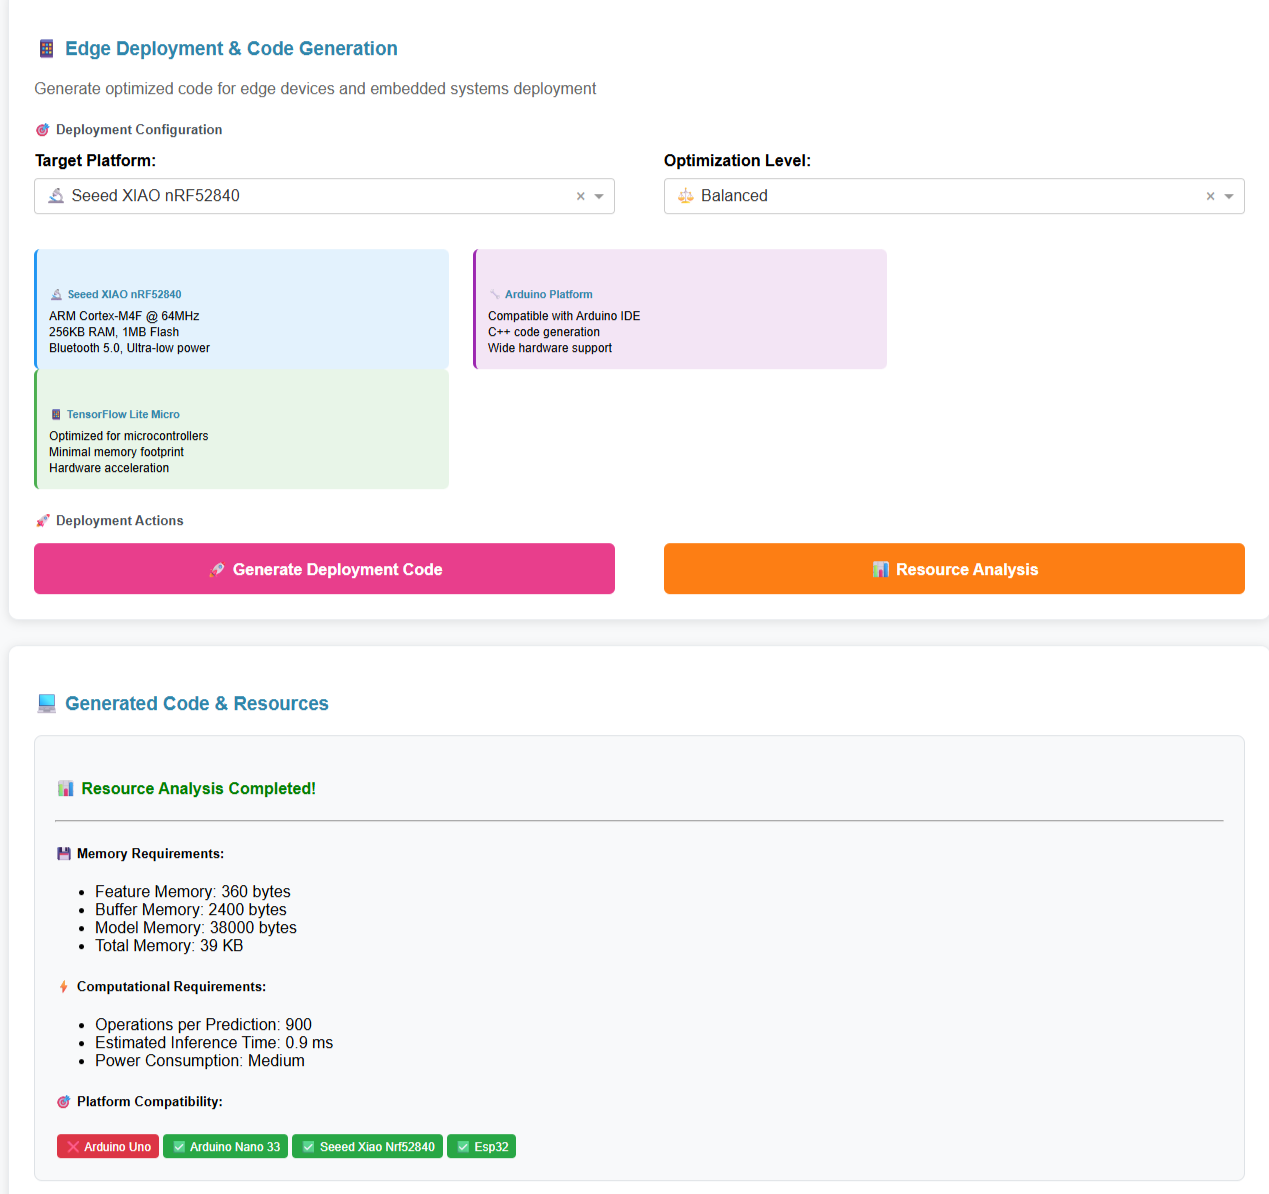
\includegraphics[width=0.95\textwidth]{figures/ui_code_generation.png}
    \caption{Giao diện tạo mã triển khai. Hiển thị các tệp header, implementation và Arduino sketch được sinh ra. Người dùng chọn chế độ tối ưu hóa (Accuracy, Speed, Power, Balanced), cấu hình nền tảng đích và tải xuống gói triển khai hoàn chỉnh.}
    \label{fig:ui_code_generation}
\end{figure}

\subsection{Kiến trúc đa mô hình: CNN code generation}
\label{subsec:cnn_code_generation}

CNN deployment khác với traditional ML vì không cần feature extraction—model nhận raw sensor data trực tiếp. Code generator cho CNN phải sinh:

\paragraph{Conv1D kernel implementation}
\begin{verbatim}
// Generated convolution kernel
void conv1d_layer1(float* input, float* output) {
    // input: [6 channels, 150 timesteps]
    // kernel: [32 filters, 6 channels, 5 timesteps]
    // output: [32 channels, 146 timesteps]
    
    for (int f = 0; f < 32; f++) {  // for each output filter
        for (int t = 0; t < 146; t++) {  // for each output timestep
            float sum = 0.0;
            for (int c = 0; c < 6; c++) {  // for each input channel
                for (int k = 0; k < 5; k++) {  // for each kernel position
                    sum += input[c*150 + t+k] * KERNEL[f][c][k];
                }
            }
            output[f*146 + t] = relu(sum + BIAS[f]);
        }
    }
}
\end{verbatim}

\paragraph{Conv2D kernel (HARCNN2D)}
HARCNN2D sử dụng Conv2D với kernel shape \texttt{(3, n\_channels)} để học correlation cross-channel:
\begin{verbatim}
// input: [1, 150 timesteps, 6 channels] (reshaped 2D grid)
// kernel: [32 filters, 1 channel, 3 rows, 6 cols]
void conv2d_layer1(float input[150][6], float output[148][32]) {
    for (int f = 0; f < 32; f++) {
        for (int t = 0; t < 148; t++) {
            float sum = 0.0;
            for (int kr = 0; kr < 3; kr++) {  // kernel height
                for (int kc = 0; kc < 6; kc++) {  // kernel width (all channels)
                    sum += input[t+kr][kc] * KERNEL[f][kr][kc];
                }
            }
            output[t][f] = relu(sum + BIAS[f]);
        }
    }
}
\end{verbatim}

\paragraph{MaxPooling và Fully Connected}
\begin{verbatim}
void maxpool1d(float* input, int in_len, float* output, int pool_size) {
    for (int i = 0; i < in_len / pool_size; i++) {
        float max_val = input[i * pool_size];
        for (int j = 1; j < pool_size; j++) {
            if (input[i*pool_size + j] > max_val)
                max_val = input[i*pool_size + j];
        }
        output[i] = max_val;
    }
}

void fully_connected(float* input, float* output, int in_size, int out_size) {
    for (int o = 0; o < out_size; o++) {
        float sum = FC_BIAS[o];
        for (int i = 0; i < in_size; i++) {
            sum += input[i] * FC_WEIGHTS[o][i];
        }
        output[o] = sum;
    }
}
\end{verbatim}

\paragraph{Scaler bypass cho CNN}
Một phát hiện quan trọng trong quá trình phát triển: StandardScaler được huấn luyện trên \textit{features} (mean, std, etc.) không nên áp dụng lên \textit{raw sensor values} (input của CNN). Nếu áp dụng, phép chuẩn hóa sẽ clamp các giá trị gyro vào range $[-10, 10]$ rad/s, phá hủy thông tin tín hiệu. Framework thêm flag \texttt{skip\_scaler} trong CNN generator:

\begin{verbatim}
if model_type in ['pytorch_cnn', 'pytorch_cnn2d']:
    # CNN receives raw sensor data, do NOT apply scaler
    # Only clamp to sensor physical range if needed
    pass
else:
    # Traditional ML: apply scaler trained on features
    apply_scaler(features);
\end{verbatim}

Giải pháp này tiết kiệm 7KB Flash và loại bỏ hoàn toàn nguy cơ inference sai do scaler distortion.

\section{Module kiểm tra thiết bị}
\label{sec:device_testing_module}

Module này (Tab 6) cung cấp giao diện kết nối với thiết bị đã flash mã triển khai để xác minh hoạt động real-time.

\subsection{Giao tiếp serial}
\label{subsec:serial_communication}

Framework sử dụng \texttt{pyserial} để mở kết nối serial với thiết bị:
\begin{verbatim}
import serial

ser = serial.Serial(port='COM3', baudrate=115200, timeout=1)
while True:
    line = ser.readline().decode('utf-8').strip()
    # Parse device output: "Predicted: walking, Confidence: 0.87"
\end{verbatim}

Arduino sketch output format:
\begin{verbatim}
Predicted: <class_name>, Confidence: <max_prob>, Raw: [<prob_0>, ..., <prob_N>]
\end{verbation}

Callback nhận line, parse ra class\_name và confidence, sau đó cập nhật UI real-time.

\subsection{Hiển thị phân loại real-time}
\label{subsec:realtime_classification_display}

Giao diện hiển thị:
\begin{itemize}
    \item \textbf{Predicted activity}: tên hoạt động dự đoán với màu sắc tương ứng.
    \item \textbf{Confidence bar}: thanh ngang hiển thị xác suất của class được dự đoán (0--100\%).
    \item \textbf{Probability distribution}: bar chart hiển thị xác suất của tất cả classes, giúp phát hiện ambiguous cases (nhiều classes có prob gần bằng nhau).
    \item \textbf{Timeline}: biểu đồ thời gian hiển thị lịch sử dự đoán 30 giây gần nhất, cho thấy transition giữa các hoạt động.
\end{itemize}

\subsection{Ngưỡng tin cậy}
\label{subsec:confidence_threshold}

Framework sinh mã có confidence thresholding: nếu \texttt{max(probabilities) < threshold}, mô hình trả về \texttt{UNKNOWN} thay vì dự đoán một class với tin cậy thấp. Điều này quan trọng cho deployment thực tế khi gặp hoạt động ngoài tập training (out-of-distribution).

\begin{verbatim}
// Generated C++ code with confidence threshold
int predict_with_confidence(float* features, float threshold) {
    float probs[NUM_CLASSES];
    compute_probabilities(features, probs);
    
    int max_class = 0;
    float max_prob = probs[0];
    for (int i = 1; i < NUM_CLASSES; i++) {
        if (probs[i] > max_prob) {
            max_prob = probs[i];
            max_class = i;
        }
    }
    
    if (max_prob < threshold) {
        return -1;  // UNKNOWN
    }
    return max_class;
}
\end{verbatim}

Người dùng có thể điều chỉnh threshold trong giao diện (mặc định: 0.7).

\subsection{Quy trình xác minh triển khai}
\label{subsec:deployment_verification_workflow}

Workflow kiểm thử trên thiết bị:
\begin{enumerate}
    \item \textbf{Flash code}: upload mã sinh ra lên vi điều khiển qua Arduino IDE hoặc PlatformIO.
    \item \textbf{Connect serial}: mở Tab 6, chọn COM port, kết nối.
    \item \textbf{Perform activities}: thực hiện các hoạt động từ tập training (VD: đứng yên, đi bộ, chạy).
    \item \textbf{Verify predictions}: so sánh dự đoán của thiết bị với ground truth.
    \item \textbf{Test edge cases}: thực hiện hoạt động ngoài tập training (VD: nhảy, đạp xe) để kiểm tra UNKNOWN detection.
    \item \textbf{Measure latency}: framework hiển thị thời gian xử lý mỗi window (từ thu thập sensor đến xuất kết quả).
\end{enumerate}

Nếu phát hiện mismatch giữa dự đoán Python và thiết bị, framework cung cấp công cụ debugging:
\begin{itemize}
    \item \textbf{Feature comparison}: xuất features từ thiết bị qua serial, so sánh với Python.
    \item \textbf{Parity validator}: kiểm tra từng bước trong pipeline (magnitude computation, statistical features, scaler, prediction).
\end{itemize}

\section{Luồng dữ liệu và quản lý trạng thái tổng thể}
\label{sec:dataflow_state_management}

\subsection{Luồng dữ liệu end-to-end}
\label{subsec:end_to_end_dataflow}

Dữ liệu chảy qua framework theo pipeline rõ ràng:

\begin{enumerate}
    \item \textbf{CSV upload (Tab 1)}:
    \begin{itemize}
        \item Input: user uploads CSV files
        \item Output: \texttt{persistent\_data/datasets/\{activity\}.csv}
        \item State: metadata (columns, sampling rate) → \texttt{dcc.Store}
    \end{itemize}
    
    \item \textbf{Preprocessing (Tab 2)}:
    \begin{itemize}
        \item Input: read CSVs from \texttt{datasets/}
        \item Process: user selects segments via drag-and-drop
        \item Output: sliding windows → \texttt{persistent\_data/windows/\{dataset\_name\}.pkl}
        \item State: segments list → \texttt{dcc.Store}
    \end{itemize}
    
    \item \textbf{Feature Engineering (Tab 3)}:
    \begin{itemize}
        \item Input: load windows from \texttt{windows/\{dataset\_name\}.pkl}
        \item Process: extract features, augmentation, train/val/test split
        \item Output: \texttt{persistent\_data/training/\{dataset\_name\}\_train.csv}, \texttt{\_val.csv}, \texttt{\_test.csv}
        \item State: feature mode, augmentation config → saved in CSV metadata
    \end{itemize}
    
    \item \textbf{Training (Tab 4)}:
    \begin{itemize}
        \item Input: load feature matrices from \texttt{training/*.csv}
        \item Process: GridSearchCV, fit model, evaluate
        \item Output: \texttt{persistent\_data/models/\{model\_name\}.joblib}
        \item State: training metrics → dashboard display
    \end{itemize}
    
    \item \textbf{Code Generation (Tab 5)}:
    \begin{itemize}
        \item Input: load model from \texttt{models/\{model\_name\}.joblib}
        \item Process: extract parameters, reorder features, render templates
        \item Output: \texttt{persistent\_data/generated/\{model\_type\}\_models/\{model\_name\}/} (header, cpp, ino)
        \item State: optimization mode, platform → \texttt{dcc.Store}
    \end{itemize}
    
    \item \textbf{Device Testing (Tab 6)}:
    \begin{itemize}
        \item Input: serial communication với flashed device
        \item Process: parse predictions, compare with expected
        \item Output: real-time dashboard, logging
        \item State: serial port, threshold → \texttt{dcc.Store}
    \end{itemize}
\end{enumerate}

\subsection{Cơ chế rollback và retry}
\label{subsec:rollback_retry}

Một ưu điểm của thiết kế filesystem-based state management là người dùng có thể quay lại bất kỳ bước nào để điều chỉnh mà không mất công việc đã hoàn thành:

\paragraph{Ví dụ 1: Thay đổi feature mode}
Nếu người dùng huấn luyện model với \texttt{time\_domain} (90 features) nhưng muốn thử \texttt{orientation\_invariant} (33 features):
\begin{enumerate}
    \item Quay lại Tab 3, chọn \texttt{orientation\_invariant}.
    \item Re-run feature extraction → sinh \texttt{*\_train.csv} mới.
    \item Quay lại Tab 4, retrain model trên features mới.
\end{enumerate}
Windows đã sinh (Tab 2) được giữ nguyên, không cần re-select segments.

\paragraph{Ví dụ 2: Điều chỉnh hyperparameters}
Nếu GridSearchCV không cho kết quả tốt, người dùng có thể:
\begin{enumerate}
    \item Mở rộng param grid (VD: thêm \texttt{max\_depth: [30, 50]} cho Random Forest).
    \item Re-run training với param grid mới.
    \item So sánh metrics giữa các models đã huấn luyện (tất cả \texttt{.joblib} files đều được giữ lại).
\end{enumerate}

\paragraph{Ví dụ 3: Deployment target mới}
Nếu muốn triển khai model đã huấn luyện lên ESP32 thay vì XIAO:
\begin{enumerate}
    \item Quay lại Tab 5, chọn platform = \texttt{ESP32}, backend = \texttt{MicroPython}.
    \item Re-run code generation → sinh MicroPython code mới.
    \item Không cần retrain model.
\end{enumerate}

\subsection{Truy xuất thông tin model}
\label{subsec:model_introspection}

Mỗi \texttt{.joblib} file chứa đầy đủ thông tin để reproduce và introspect:
\begin{itemize}
    \item \texttt{feature\_names}: biết chính xác features nào được sử dụng.
    \item \texttt{model\_params}: biết hyperparameters đã chọn.
    \item \texttt{performance\_metrics}: so sánh accuracy giữa các models.
    \item \texttt{scaler}: có thể transform new data với cùng scaler.
\end{itemize}

Framework cung cấp utility function để load và inspect model:
\begin{verbatim}
import joblib

def inspect_model(model_path):
    model_data = joblib.load(model_path)
    print(f"Model type: {model_data['model_type']}")
    print(f"Features ({len(model_data['feature_names'])}): {model_data['feature_names']}")
    print(f"Classes: {list(model_data['label_encoder'].classes_)}")
    print(f"Test accuracy: {model_data['performance_metrics']['accuracy']:.4f}")
    print(f"Hyperparameters: {model_data['model_params']}")
\end{verbatim}

\section{Tổng kết chương}
\label{sec:design_implementation_summary}

Chương này trình bày chi tiết kiến trúc hệ thống và hiện thực kỹ thuật của framework HAR Edge Deployment. Các điểm chính:

\begin{enumerate}
    \item \textbf{Kiến trúc module hóa}: hệ thống được tổ chức thành 6 modules độc lập tương ứng với 6 tabs, mỗi module chịu trách nhiệm một giai đoạn rõ ràng trong pipeline.
    
    \item \textbf{State management hybrid}: kết hợp filesystem persistence (cho dữ liệu trung gian) và in-memory state (cho session-specific metadata), cho phép rollback và retry linh hoạt.
    
    \item \textbf{Code generation architecture}: factory pattern + block-based clean architecture, hỗ trợ ma trận 3 chiều (model × platform × backend) mà vẫn duy trì tính module.
    
    \item \textbf{Training-deployment parity}: các cơ chế bảo đảm nhất quán (feature reordering, scaler bypass cho CNN, confidence thresholding) đảm bảo mô hình hoạt động đúng trên thiết bị.
    
    \item \textbf{User experience}: giao diện tương tác (drag-and-drop, real-time monitoring) giảm thiểu barrier to entry, cho phép người dùng không chuyên về embedded systems vẫn triển khai được edge ML.
\end{enumerate}

Chương tiếp theo sẽ trình bày kết quả thực nghiệm, đo lường hiệu năng trên Seeed XIAO nRF52840, và so sánh với các nền tảng thương mại.
